\section{Konvexe Hülle}
\writtenby{\dcauthornameewie}%
Als konvexe Hülle einer Punktmenge $M$ bezeichnet man das minimale konvexe Polygon, welches sämtliche Punkte aus $M$ enthält.
Für die Berechnung der konvexen Hülle aus einer Menge von Punkten existieren diverse Alogirthmen.
Ein simpler Algorithmus ist \textsc{Andrew}'s Monotone Chain  \cite[6--7]{compgeom2008}.
Dazu werden zwei "`halbe"' Hüllen erstellt, die obere Hülle $U$ und untere Hülle $L$.
Die obere Hülle wird erzeugt indem über alle Punkte der Menge $M$ entsprechend ihrer lexikografischen Ordnung\footnote{
  \( (x,y) < (u, v) \Longleftrightarrow x < u \vee x = u \wedge y < v \)
} iteriert, und wiederholt das letzte Element in $U$ entfernt wird solange $U$ mindestens 2 Punkte enthält und die letzten 2 Punkte zusammen mit dem aktuell betrachteten Punkt keine Rechtskurve bilden.
Anschließend wird der aktuelle Punkt ans Ende von $U$ eingefügt.
Die Erzeugung der unteren Hülle $L$ erfolgt analog $U$, jedoch unter Betrachtung der Punkte in umgekehrter Reihenfolge.
Zudem müssen die letzten 2 Punkte zusammen mit dem aktuell betrachteten Punkt eine Rechtskurve bilden.
Abschließend werden $U$ und $L$ so zusammen gefasst, dass diese die konvexe Hülle als Liste von Eckpunkten im Uhrzeigersinn ergeben.

\begin{figure}[H]
  \centering
  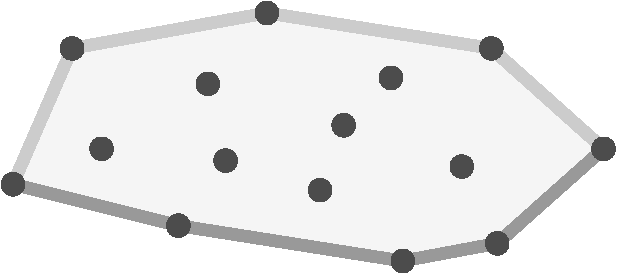
\includegraphics[width=0.5\columnwidth]{img/basics/convex-hull/andrews-monotone-chain}
  \caption[\textsc{Andrew}'s Monotone Chain]{\textsc{Andrew}'s Monotone Chain mit oberer Hülle $U$ (hellgrau) und unterer Hülle $L$ (dunkelgrau)}
\end{figure}
